\documentclass[11pt,a4paper]{article}
\usepackage{gtu-el-yazisi}
\begin{document}
\notbilgi{İşaretler ve Sistemler}{Ders 2 -- Birim dürtü ve birim basamak fonksiyonları, sistem özellikleri}{Isaret-ve-Sistemler-ders-2.pdf}
\renewcommand{\thempfootnote}{\alph{mpfootnote}} % kutu içi dipnotlar için (euler + \itshape uyumsuzluğu)

\section{Birim Dürtü ve Birim Basamak Fonksiyonları}
\sayfa{1}
(Unit Impulse and Unit Step Functions)

\subsection{Ayrık zamanlı birim dürtü işareti:}
\noindent
\begin{minipage}[c]{0.45\linewidth}
\[ \delta[n] = \begin{cases} 1, & n = 0 \\ 0, & n \neq 0 \end{cases} \]
\end{minipage}\hfill
\begin{minipage}[c]{0.5\linewidth}
\centering
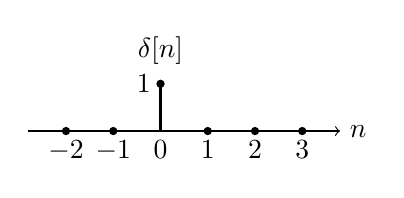
\begin{tikzpicture}[scale=0.6]
  \draw[->] (-2.8,0) -- (3.8,0) node[right] {$n$};
  \foreach \x in {-2,-1,1,2,3} { \fill (\x,0) circle (2.5pt); \node[below] at (\x,0) {$\x$}; }
  \draw[thick] (0,0) -- (0,1); \fill (0,1) circle (2.5pt);
  \node[below] at (0,0) {$0$};
  \node[left] at (0,1) {$1$};
  \node[above] at (0,1.2) {$\delta[n]$};
\end{tikzpicture}
\end{minipage}

\subsection{Ayrık zamanlı birim basamak işareti:}
\noindent
\begin{minipage}[c]{0.45\linewidth}
\[ u[n] = \begin{cases} 1, & n \geq 0 \\ 0, & n < 0 \end{cases} \]
\end{minipage}\hfill
\begin{minipage}[c]{0.5\linewidth}
\centering
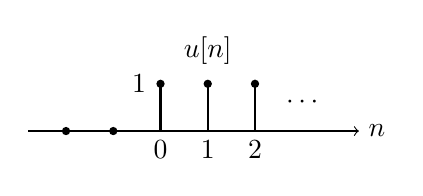
\begin{tikzpicture}[scale=0.6]
  \draw[->] (-2.8,0) -- (4.2,0) node[right] {$n$};
  \foreach \x in {-2,-1} { \fill (\x,0) circle (2.5pt); }
  \foreach \x in {0,1,2} { \draw[thick] (\x,0) -- (\x,1); \fill (\x,1) circle (2.5pt); \node[below] at (\x,0) {$\x$}; }
  \node at (3,0.6) {$\cdots$};
  \node[left] at (-0.1,1) {$1$};
  \node[above] at (1,1.2) {$u[n]$};
\end{tikzpicture}
\end{minipage}

\medskip
$\Rightarrow$ Birim dürtü ve birim basamak fonksiyonları arasındaki ilişki

\noindent
\begin{minipage}[c]{0.5\linewidth}
\textcolor{kirmizikalem}{\textbf{\Large !}}\quad
$\ast\ \delta[n] = u[n] - u[n-1]$
\end{minipage}\hfill
\begin{minipage}[c]{0.46\linewidth}
\centering
\begin{tikzpicture}[scale=0.6]
  \draw (-1,0) -- (6,0);
  \foreach \x/\p in {0/0,1/1.3,2/2.6,3/3.9} { \draw[thick] (\p,0) -- (\p,1); \fill (\p,1) circle (2.5pt); \node[below] at (\p,0) {$\x$}; }
  \draw[dashed, kursunkalem] (0,1) -- (3.9,1);
  \node at (5.1,0.5) {$\cdots$};
  \node[above left] at (0.3,1.1) {\small $u[n]$};
  \node[above right] at (0.9,1.1) {\small $u[n-1]$};
\end{tikzpicture}
\end{minipage}

\medskip
\noindent
\begin{minipage}[c]{0.62\linewidth}
\textcolor{turuncukalem}{$\blacktriangleright$}\ $\ast\ u[n] = \sum\limits_{k=0}^{\infty} \delta[n-k] = \delta[n] + \delta[n-1] + \delta[n-2] + \cdots$
\end{minipage}\hfill
\begin{minipage}[c]{0.36\linewidth}
\centering
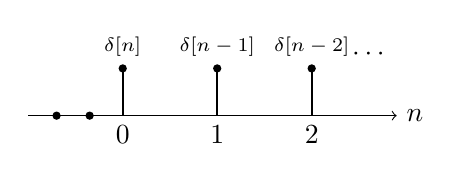
\begin{tikzpicture}[scale=0.6]
  \draw[->] (-2,0) -- (5.8,0) node[right] {$n$};
  \fill (-1.4,0) circle (2.5pt); \fill (-0.7,0) circle (2.5pt);
  \foreach \x/\l/\p in {0/{\delta[n]}/0,1/{\delta[n-1]}/2,2/{\delta[n-2]}/4} { \draw[thick] (\p,0) -- (\p,1); \fill (\p,1) circle (2.5pt); \node[below] at (\p,0) {$\x$}; \node[above] at (\p,1.05) {\scriptsize $\l$}; }
  \node at (5.2,1.3) {$\cdots$};
\end{tikzpicture}
\end{minipage}

\medskip
$\Rightarrow$ Birim dürtü işaretinin örnekleme özelliği
\begin{align*}
  x[n]\,\delta[n] &= x[0]\,\delta[n] \\
  x[n]\,\delta[n-n_0] &= x[n_0]\,\delta[n-n_0]
\end{align*}

\subsection{Sürekli zamanlı birim basamak işareti:}
\noindent
\begin{minipage}[c]{0.45\linewidth}
\[ u(t) = \begin{cases} 1, & t > 0 \\ 0, & t < 0 \end{cases} \]
\end{minipage}\hfill
\begin{minipage}[c]{0.5\linewidth}
\centering
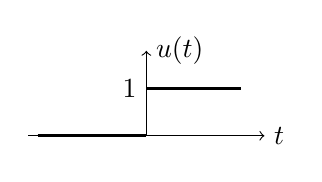
\begin{tikzpicture}[scale=0.6]
  \draw[->] (-2.5,0) -- (2.5,0) node[right] {$t$};
  \draw[->] (0,0) -- (0,1.8) node[right] {$u(t)$};
  \draw[very thick] (-2.3,0) -- (0,0);
  \draw[thick] (0,1) -- (2,1);
  \node[left] at (0,1) {$1$};
\end{tikzpicture}
\end{minipage}

\noindent
\begin{minipage}[c]{0.45\linewidth}
Lathi: \quad $u(t) = \begin{cases} 1, & t \geq 0 \\ 0, & t < 0 \end{cases}$
\end{minipage}\hfill
\begin{minipage}[c]{0.5\linewidth}
\centering
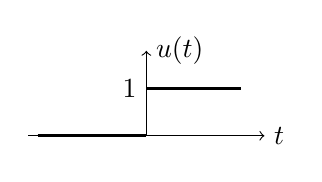
\begin{tikzpicture}[scale=0.6]
  \draw[->] (-2.5,0) -- (2.5,0) node[right] {$t$};
  \draw[->] (0,0) -- (0,1.8) node[right] {$u(t)$};
  \draw[very thick] (-2.3,0) -- (0,0);
  \draw[thick] (0,1) -- (2,1);
  \node[left] at (0,1) {$1$};
\end{tikzpicture}
\end{minipage}

\subsection{Sürekli zamanlı birim dürtü işareti:}
\sayfa{2}
\noindent
\begin{minipage}[c]{0.36\linewidth}
\[ \delta(t) = \begin{cases} \infty, & t = 0 \\ 0, & t \neq 0 \end{cases} \]
\end{minipage}\hfill
\begin{minipage}[c]{0.3\linewidth}
\[ \int_{-\infty}^{\infty} \delta(t)\,dt = 1 \]
\end{minipage}\hfill
\begin{minipage}[c]{0.3\linewidth}
\centering
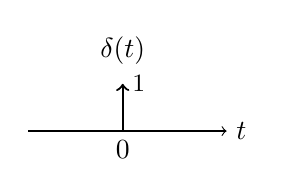
\begin{tikzpicture}[scale=0.6]
  \draw[->] (-2,0) -- (2.2,0) node[right] {$t$};
  \draw[->, thick] (0,0) -- (0,1);
  \node[right] at (0,1) {\small $1$};
  \node[above] at (0,1.2) {$\delta(t)$};
  \node[below] at (0,0) {$0$};
\end{tikzpicture}
\end{minipage}

\smallskip
Sürekli zamanlı birim dürtü işareti, $t=0$ iken $\infty$'a giden ve alanı $1$'e eşit olan bir fonksiyondur.

\[ \ast\ u(t) = \int_{-\infty}^{t} \delta(\tau)\,d\tau \]
\[ \ast\ \delta(t) = \frac{du(t)}{dt} \]
\begin{align*}
  \ast\ x(t)\,\delta(t) &= x(0)\,\delta(t) \\
  x(t)\,\delta(t-t_0) &= x(t_0)\,\delta(t-t_0)
\end{align*}

$\ast$\ $x(t)$, $t=t_0$'da sürekli olmak üzere
\[ \int_{a}^{b} x(t)\,\delta(t-t_0)\,dt = \begin{cases} x(t_0), & a < t_0 < b \\ 0, & \text{diğer} \end{cases} \]

\[ \ast\ \delta(at) = \frac{1}{|a|}\,\delta(t), \quad \forall a \neq 0 \]
$a=-1$ için $\delta(-t) = \delta(t)$ : Çift fonksiyon

\begin{ornek}[(Ex)]
$x(t) = \delta(t+2) - \delta(t-2)$
\[ y(t) = \int_{-\infty}^{t} x(\tau)\,d\tau, \qquad E_y = ? \quad P_y = ? \]
\end{ornek}
\begin{cozum}
\[ y(t) = \int_{-\infty}^{t} \bigl[\delta(\tau+2) - \delta(\tau-2)\bigr]\,d\tau = \int_{-\infty}^{t} \delta(\tau+2)\,d\tau - \int_{-\infty}^{t} \delta(\tau-2)\,d\tau = u(t+2) - u(t-2) \]
\[ y(t) = \begin{cases} 0, & t < -2 \\ 1, & -2 \leq t \leq 2 \\ 0, & t > 2 \end{cases} \]
\[ E_y = \int_{-\infty}^{\infty} |y(t)|^2\,dt = \int_{-2}^{2} 1\cdot dt = 4 \]
\[ P_y = \lim_{T\to\infty} \frac{1}{2T} \int_{-T}^{T} |y(t)|^2\,dt = 0 \]
\end{cozum}

\begin{ornek}[(Ex)]
\sayfa{3}
$x(t) = \mathrm{Even}\bigl\{\sin(4\pi t)\,u(t)\bigr\}$ \quad Periyodik midir?
\end{ornek}
\begin{cozum}
Reminder: \ $\mathrm{Even}\{x(t)\} = x_e(t) = \dfrac{x(t) + x(-t)}{2}$
\[ x(t) = \frac{\sin(4\pi t)\,u(t) + \sin(-4\pi t)\,u(-t)}{2} = \frac{1}{2}\bigl[\sin(4\pi t)\,u(t) - \sin(4\pi t)\,u(-t)\bigr] \]
\[ x(t) = \frac{1}{2}\sin(4\pi t)\,\bigl[u(t) - u(-t)\bigr] \]

\noindent
\begin{minipage}[c]{0.32\linewidth}
\centering
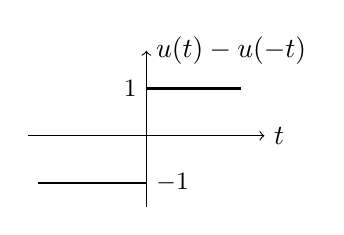
\begin{tikzpicture}[scale=0.6]
  \draw[->] (-2.5,0) -- (2.5,0) node[right] {$t$};
  \draw[->] (0,-1.5) -- (0,1.8) node[right] {$u(t)-u(-t)$};
  \draw[thick] (0,1) -- (2,1);
  \draw[thick] (-2.3,-1) -- (0,-1);
  \node[left] at (0,1) {\small $1$};
  \node[right] at (0,-1) {\small $-1$};
\end{tikzpicture}
\end{minipage}\hfill
\begin{minipage}[c]{0.64\linewidth}
\[ u(t) - u(-t) = \begin{cases} 1, & t > 0 \\ -1, & t < 0 \\ 0, & t = 0 \end{cases} \qquad = \mathrm{sgn}(t) \ \text{ işaret fonksiyonu} \]
\end{minipage}

\[ x(t) = \frac{1}{2}\sin(4\pi t)\,\mathrm{sgn}(t) \qquad \text{Nonperiodic} \]
\end{cozum}

\begin{ornek}
$x(t) = A\cos(\omega_0 t + \theta)$, \quad $E_x = ?$, \ $P_x = ?$, \quad $\omega_0 = \dfrac{2\pi}{T}$
\end{ornek}
\begin{cozum}
\begin{align*}
  E_x &= \lim_{T\to\infty} \int_{-T}^{T} |x(t)|^2\,dt = \lim_{T\to\infty} \int_{-T}^{T} A^2\cos^2(\omega_0 t + \theta)\,dt \\
  &= \lim_{T\to\infty} \int_{-T}^{T} \frac{A^2}{2}\bigl[1 + \cos(2\omega_0 t + 2\theta)\bigr]\,dt \\
  &= \lim_{T\to\infty} \frac{A^2}{2}\left[t + \frac{\sin(2\omega_0 t + 2\theta)}{2\omega_0}\right]\Bigg|_{-T}^{T} \\
  &= \lim_{T\to\infty} \frac{A^2}{2}\left[2T + \frac{1}{2\omega_0}\Bigl(\sin(2\omega_0 T + 2\theta) - \sin(-2\omega_0 T + 2\theta)\Bigr)\right] \longrightarrow \infty
\end{align*}
\begin{align*}
  P_x &= \lim_{T\to\infty} \frac{1}{2T} \int_{-T}^{T} |x(t)|^2\,dt \\
  &= \lim_{T\to\infty} \frac{1}{2T}\,\frac{A^2}{2}\Biggl[2T + \frac{T}{4\pi}\underbrace{\Bigl(\underbrace{\sin(4\pi + 2\theta)}_{\sin 2\theta} - \underbrace{\sin(-4\pi + 2\theta)}_{\sin 2\theta}\Bigr)}_{=\,0}\Biggr] = \lim_{T\to\infty} \frac{A^2}{2} = \frac{A^2}{2}
\end{align*}
\end{cozum}

$\ast$ Periyodik işaretler güç işaretidir \ ($0 < P_x < \infty$, \ $E_x \to \infty$).

\sayfa{4}
\textbf{\underline{Sistem:}} Girişine uygulanan işarete karşılık çıkışında uygun bir işaret üreten düzenektir.

\begin{center}
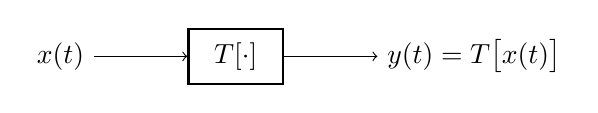
\begin{tikzpicture}
  \node[draw, thick, minimum width=1.2cm, minimum height=0.7cm] (T) at (0,0) {$T[\cdot]$};
  \draw[->] (-1.8,0) node[left] {$x(t)$} -- (T.west);
  \draw[->] (T.east) -- (1.8,0) node[right] {$y(t) = T\bigl[x(t)\bigr]$};
\end{tikzpicture}
\end{center}

\textbf{\underline{Sürekli zamanlı sistem:}} Giriş ve çıkış işaretlerinin her ikisi de sürekli zamanlıdır.

\begin{center}
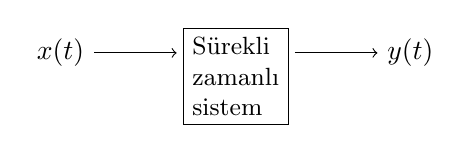
\begin{tikzpicture}
  \node[draw, align=left, font=\small] (S) at (0,0) {Sürekli\\zamanlı\\sistem};
  \draw[->] (-1.8,0.3) node[left] {$x(t)$} -- (-0.75,0.3);
  \draw[->] (0.75,0.3) -- (1.8,0.3) node[right] {$y(t)$};
\end{tikzpicture}
\end{center}

\textbf{\underline{Ayrık zamanlı sistem:}} Giriş, çıkış işaretlerinin her ikisi de ayrık zamanlıdır.

\begin{center}
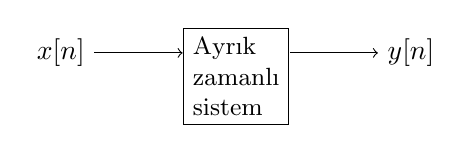
\begin{tikzpicture}
  \node[draw, align=left, font=\small] (S) at (0,0) {Ayrık\\zamanlı\\sistem};
  \draw[->] (-1.8,0.3) node[left] {$x[n]$} -- (-0.68,0.3);
  \draw[->] (0.68,0.3) -- (1.8,0.3) node[right] {$y[n]$};
\end{tikzpicture}
\end{center}

\begin{ornek}[(Ex)]
\noindent
\begin{minipage}[c]{0.3\linewidth}
\centering
\begin{circuitikz}
  \draw (0,0) to[V, l=$V_s$] (0,2) to[R, l_=$R$] (2.6,2) to[C] (2.6,0) -- (0,0);
  \node at (2.95,1.25) {\scriptsize $+$};
  \node at (2.95,0.75) {\scriptsize $-$};
  \node[right] at (3.05,1) {$V_c$};
  \draw[->] (0.75,1.25) arc[start angle=160, end angle=20, radius=0.55];
  \node at (1.6,0.55) {\small $i(t)$};
\end{circuitikz}
\end{minipage}\hfill
\begin{minipage}[c]{0.66\linewidth}
$V_c(t)$: çıkış işareti\\
$V_s(t)$: giriş işareti
\[ i(t) = \frac{V_s(t) - V_c(t)}{R} = \frac{1}{C}\frac{dV_c(t)}{dt} \;\Rightarrow\; \frac{dV_c(t)}{dt} + \frac{1}{RC}V_c(t) = \frac{1}{RC}V_s(t) \quad \text{\footnotemark} \]
\end{minipage}
\end{ornek}
\footnotetext{Claude notu: muhtemelen $i(t) = C\,\frac{dV_c(t)}{dt}$ olmalı ($\frac{1}{C}$ değil); son diferansiyel denklem doğru.}

\subsection{$\Rightarrow$ Sistemlerin birbirine bağlanması}
$\ast$ \textbf{Seri} (series or cascade) bağlama

\begin{center}

\begin{tikzpicture}
  \node[draw, minimum height=0.6cm] (A) at (0,0) {sistem 1};
  \node[draw, minimum height=0.6cm] (B) at (2.6,0) {sistem 2};
  \draw[->] (-1.9,0) node[left] {Giriş} -- (A.west);
  \draw[->] (A.east) -- (B.west);
  \draw[->] (B.east) -- (4.3,0) node[right] {$\cdots$};
  \draw[->] (4.9,0) -- (5.8,0) node[right] {Çıkış};
\end{tikzpicture}
\end{center}

Seri bağlı sistemlerde sistemlerin bağlanma sırası önemlidir.

\begin{ornek}[(Ex)]
\begin{center}
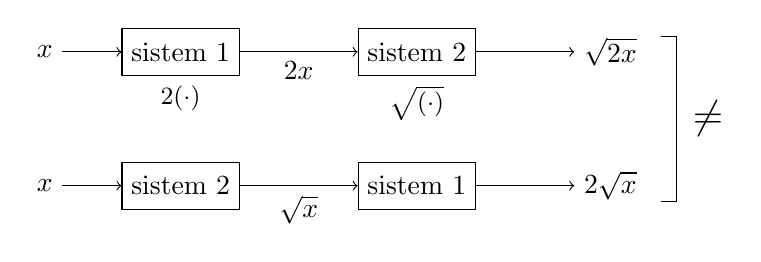
\begin{tikzpicture}
  \node[draw, minimum height=0.6cm] (A1) at (0,0) {sistem 1};
  \node[below] at (A1.south) {\small $2(\cdot)$};
  \node[draw, minimum height=0.6cm] (B1) at (3,0) {sistem 2};
  \node[below] at (B1.south) {\small $\sqrt{(\cdot)}$};
  \draw[->] (-1.5,0) node[left] {$x$} -- (A1.west);
  \draw[->] (A1.east) -- node[below] {$2x$} (B1.west);
  \draw[->] (B1.east) -- (5,0) node[right] {$\sqrt{2x}$};
  \node[draw, minimum height=0.6cm] (B2) at (0,-1.7) {sistem 2};
  \node[draw, minimum height=0.6cm] (A2) at (3,-1.7) {sistem 1};
  \draw[->] (-1.5,-1.7) node[left] {$x$} -- (B2.west);
  \draw[->] (B2.east) -- node[below] {$\sqrt{x}$} (A2.west);
  \draw[->] (A2.east) -- (5,-1.7) node[right] {$2\sqrt{x}$};
  \draw (6.1,0.2) -- (6.3,0.2) -- (6.3,-1.9) -- (6.1,-1.9);
  \node at (6.7,-0.85) {\Large $\neq$};
\end{tikzpicture}
\end{center}
\end{ornek}

\noindent
\begin{minipage}[t]{0.48\linewidth}
$\ast$ \textbf{Paralel} bağlama

\centering
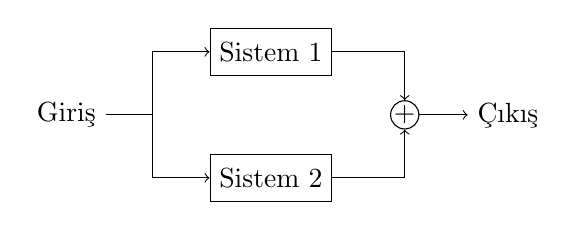
\begin{tikzpicture}
  \node[draw, minimum height=0.6cm] (A) at (1.5,0.8) {Sistem 1};
  \node[draw, minimum height=0.6cm] (B) at (1.5,-0.8) {Sistem 2};
  \node[draw, circle, inner sep=0pt, minimum size=0.35cm] (S) at (3.2,0) {$+$};
  \draw (-0.6,0) node[left] {Giriş} -- (0,0);
  \draw[->] (0,0) |- (A.west);
  \draw[->] (0,0) |- (B.west);
  \draw[->] (A.east) -| (S.north);
  \draw[->] (B.east) -| (S.south);
  \draw[->] (S.east) -- (4,0) node[right] {Çıkış};
\end{tikzpicture}
\end{minipage}\hfill
\begin{minipage}[t]{0.48\linewidth}
$\ast$ \textbf{Geri besleme} ile bağlama

\centering
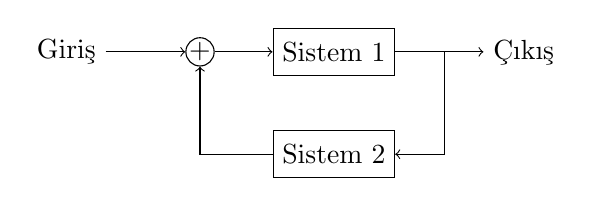
\begin{tikzpicture}
  \node[draw, circle, inner sep=0pt, minimum size=0.35cm] (S) at (0,0) {$+$};
  \node[draw, minimum height=0.6cm] (A) at (1.7,0) {Sistem 1};
  \node[draw, minimum height=0.6cm] (B) at (1.7,-1.3) {Sistem 2};
  \draw[->] (-1.2,0) node[left] {Giriş} -- (S.west);
  \draw[->] (S.east) -- (A.west);
  \draw[->] (A.east) -- (3.6,0) node[right] {Çıkış};
  \draw[->] (3.1,0) |- (B.east);
  \draw[->] (B.west) -| (S.south);
\end{tikzpicture}
\end{minipage}

\section{Sistem Özellikleri (System Properties)}
\sayfa{5}
Sistemlerin Sınıflandırılması (classification of systems)

\subsection{1) Hafızaya sahip olan ve olmayan sistemler:}
(System with and without memory)

Instantaneous (memoryless) and dynamic (with memory) systems

\textbf{Hafızası olmayan sistem:} Bir sistemin herhangi bir zamandaki çıktısı her bağımsız değişkenin sadece o andaki girdisine bağlıdır.

\begin{ornek}[(Ex)]
\begin{align*}
  y[n] &= \bigl(x[n] - x^2[n]\bigr)^2 &&: \text{memoryless} \\
  y[n] &= \sum_{k=-\infty}^{n} x[k] &&: \text{memory} \\
  y[n] &= x[n-1] &&: \text{memory} \\
  y(t) &= \int_{-\infty}^{t} x(\tau)\,d\tau &&: \text{memory} \\
  y(t) &= 2x(t) + x^3(t) &&: \text{memoryless}
\end{align*}
\end{ornek}

\subsection{2) Tersinir ve tersinir olmayan sistemler:}
(Invertible and noninvertible systems)

\textbf{Tersinir sistem:} Çıktısı verilen bir sistemin özgün girdisi bulunabiliyorsa bu sistem tersinirdir.
Bir sistem farklı girdiler için farklı çıktılar üretebiliyor ise tersinirdir.

\begin{center}
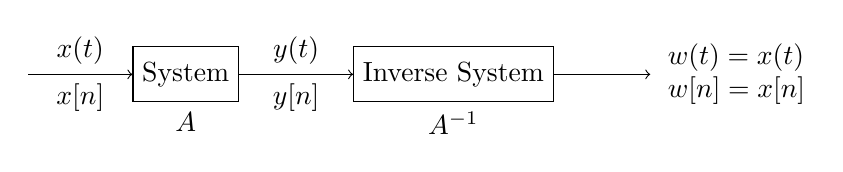
\begin{tikzpicture}
  \node[draw, minimum height=0.7cm] (A) at (0,0) {System};
  \node[below] at (A.south) {$A$};
  \node[draw, minimum height=0.7cm] (B) at (3.4,0) {Inverse System};
  \node[below] at (B.south) {$A^{-1}$};
  \draw[->] (-2,0) -- node[above] {$x(t)$} node[below] {$x[n]$} (A.west);
  \draw[->] (A.east) -- node[above] {$y(t)$} node[below] {$y[n]$} (B.west);
  \draw[->] (B.east) -- (5.9,0);
  \node[right, align=left] at (6,0) {$w(t) = x(t)$\\ $w[n] = x[n]$};
\end{tikzpicture}
\end{center}

\begin{ornek}[(Ex)]
$y(t) = 2x(t)$ sistemi tersinir midir?
\begin{center}
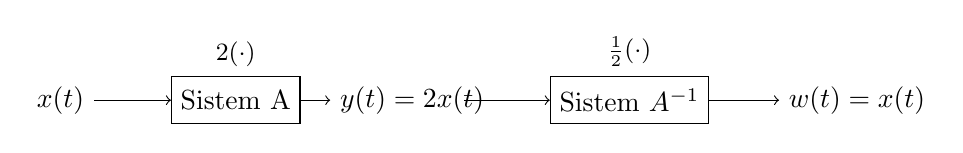
\begin{tikzpicture}
  \node[draw, minimum height=0.6cm] (A) at (0,0) {Sistem A};
  \node[above] at (A.north) {\small $2(\cdot)$};
  \node[draw, minimum height=0.6cm] (B) at (5,0) {Sistem $A^{-1}$};
  \node[above] at (B.north) {\small $\frac{1}{2}(\cdot)$};
  \draw[->] (-1.8,0) node[left] {$x(t)$} -- (A.west);
  \draw[->] (A.east) -- (1.2,0) node[right] {$y(t) = 2x(t)$};
  \draw[->] (2.9,0) -- (B.west);
  \draw[->] (B.east) -- (6.9,0) node[right] {$w(t) = x(t)$};
\end{tikzpicture}
\end{center}
Sistem A: \ $y(t) = 2x(t)$

Sistem $A^{-1}$: \ $w(t) = \frac{1}{2}y(t) = x(t)$ \quad Invertible
\end{ornek}

\begin{ornek}[(Ex)]
Sistem A: \ $y(t) = \displaystyle\int_{-\infty}^{t} x(\tau)\,d\tau$ \ (integrator)
\[ A^{-1}:\ w(t) = \frac{dy(t)}{dt} = x(t) \quad \text{(differentiator)} \quad \text{Invertible} \]
\end{ornek}

\begin{ornek}[(Ex)]
System A: \ $y(t) = x^2(t)$
\[ w(t) = \sqrt{y(t)} = |x(t)| \neq x(t) \quad \text{Noninvertible} \]
\end{ornek}

\subsection{3) Nedensel ve nedensel olmayan sistemler:}
(Causal and noncausal systems)

\sayfa{6}
\textbf{Nedensel sistem:} Bir sistemin herhangi bir andaki çıktısı, sadece o andaki ve geçmişteki girdilerine bağlı ise nedenseldir.

Sistemin çıktısı girişin gelecekteki değerlerine bağlı değildir.

$\Rightarrow$ Bir sistemin fiziki olarak gerçeklenebilmesi için nedensel olması gerekir.

Nedensel olmayan sistemler işaretlerin gerçek zamanlı olarak işlenmediği durumlarda ortaya çıkar.
\[ y(t_0) = T\bigl[x(t);\ t \leq t_0\bigr] \ : \ \text{Causal} \]

\begin{ornek}[(Ex)]
\begin{align*}
  y(t) &= x(t) - x(t-3) &&: \text{Causal} \\
  y[n] &= \frac{1}{3}\bigl[x[n-1] + x[n] + x[n+1]\bigr] &&: \text{Noncausal} \\
  y[n] &= x[-n] &&: \text{Noncausal} \\
  y(t) &= x(t)\cos(t+1) &&: \text{Causal}
\end{align*}
\end{ornek}

\subsection{4) Kararlı ve kararlı olmayan sistemler:}
(Stable and nonstable systems)

\textbf{Kararlı sistem:} Bir sistem sonlu bir girdi için sonlu bir çıkış üretiyorsa kararlıdır.
\begin{center}
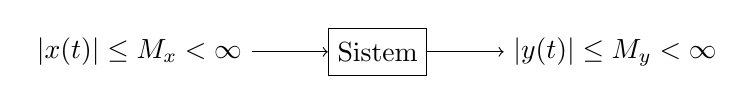
\begin{tikzpicture}
  \node[draw, minimum height=0.6cm] (S) at (0,0) {Sistem};
  \draw[->] (-1.6,0) node[left] {$|x(t)| \leq M_x < \infty$} -- (S.west);
  \draw[->] (S.east) -- (1.6,0) node[right] {$|y(t)| \leq M_y < \infty$};
\end{tikzpicture}
\end{center}

\begin{ornek}[(Ex)]
$y(t) = x^2(t)$
\begin{gather*}
  |x(t)| \leq M_x < \infty \\
  |y(t)| = |x^2(t)| = |x(t)|^2 \leq M_x^2 < \infty \quad \text{Stable}
\end{gather*}
\end{ornek}

\begin{ornek}[(Ex)]
$y(t) = t\,x(t)$
\[ |y(t)| = t\,|x(t)| \leq t\,M_x \qquad t \to \infty \quad y(t) \to \infty \quad \text{Unstable} \]
\end{ornek}

\begin{ornek}[(Ex)]
$y[n] = \displaystyle\sum_{k=-\infty}^{n} x[k]$ \ : Unstable
\end{ornek}

\subsection{5) Zamanla değişen ve değişmeyen sistemler:}
\sayfa{7}
(Time-varying and time-invariant systems)

\textbf{Zamanla değişmeyen sistem:} Giriş çıkış ilişkisi zamanla değişmeyen sistemler olup aynı giriş işareti farklı zamanlarda uygulandığında aynı çıkış işaretinin zamanda kaymış versiyonlarını üretir.
\begin{align*}
  &T\bigl[x(t)\bigr] = y(t) \\
  &T\bigl[x(t-t_0)\bigr] = y(t-t_0)\ ; \ \forall t_0,\ x(t) \qquad \text{Time-Invariant} \\[1mm]
  &x[n] \longrightarrow y[n] \\
  &x[n-n_0] \longrightarrow y[n-n_0]\ ; \ \forall n_0,\ x[n]
\end{align*}

\begin{ornek}[(Ex)]
$y(t) = \sin\bigl(x(t)\bigr)$
\begin{align*}
  &T\bigl[x(t-t_0)\bigr] \overset{?}{=} y(t-t_0) \\
  &\quad T\bigl[x(t-t_0)\bigr] = \sin\bigl(x(t-t_0)\bigr) = y(t-t_0) \qquad \text{Time-Invariant}
\end{align*}
\end{ornek}

\begin{ornek}[(Ex)]
$y(t) = x(t)\sin(t)$
\[ \left.\begin{aligned}
  T\bigl[x(t-t_0)\bigr] &= x(t-t_0)\sin(t) \\
  y(t-t_0) &= x(t-t_0)\sin(t-t_0)
\end{aligned}\ \right]\neq \quad \text{Time-variant} \]
\end{ornek}

\subsection{6) Doğrusal ve doğrusal olmayan sistemler:}
(Linear and nonlinear systems)

\textbf{Doğrusal sistem:} Sistemin birkaç giriş işaretinin lineer kombinasyonuna cevabı, o işaretlere cevabının lineer kombinasyonu ise doğrusaldır.
\begin{align*}
  y_1(t) &= T\bigl[x_1(t)\bigr] \\
  y_2(t) &= T\bigl[x_2(t)\bigr] \\
  T\bigl[a x_1(t) + b x_2(t)\bigr] &= a\,T\bigl[x_1(t)\bigr] + b\,T\bigl[x_2(t)\bigr] = a\,y_1(t) + b\,y_2(t) \qquad \text{Lineer}
\end{align*}

\begin{ornek}[(Ex)]
$y(t) = \displaystyle\int_{-\infty}^{t} x(\tau)\,d\tau$
\[ T\bigl[a x_1(t) + b x_2(t)\bigr] = \int_{-\infty}^{t} \bigl(a x_1(\tau) + b x_2(\tau)\bigr)\,d\tau = a\int_{-\infty}^{t} x_1(\tau)\,d\tau + b\int_{-\infty}^{t} x_2(\tau)\,d\tau = \underbrace{a\,y_1(t) + b\,y_2(t)}_{\text{Linear}} \]
\end{ornek}

\begin{ornek}[(Ex)]
$y(t) = x^2(t)$
\begin{align*}
  T\bigl[a x_1(t) + b x_2(t)\bigr] &= \bigl(a x_1(t) + b x_2(t)\bigr)^2 = a^2 x_1^2(t) + b^2 x_2^2(t) + 2ab\,x_1(t)\,x_2(t) \\
  &= \left.\begin{aligned} &a^2 y_1(t) + b^2 y_2(t) + 2ab\,x_1(t)\,x_2(t) \\ &a\,y_1(t) + b\,y_2(t) \end{aligned}\ \right]\neq \quad \text{Nonlinear}
\end{align*}
\end{ornek}

\begin{ornek}[(Ex)]
\sayfa{8}
$y[n] = 2x[n] + 3$ \hfill \fcolorbox{kirmizikalem}{kagitrengi}{\color{turuncukalem}\small $y_1 = 2x_1 + 3$, \ $y_2 = 2x_2 + 3$}
\[ \begin{aligned}
  T\bigl[a x_1[n] + b x_2[n]\bigr] &= 2\bigl\{a x_1[n] + b x_2[n]\bigr\} + 3 = 2a\,x_1[n] + 2b\,x_2[n] + 3 \\
  &= \left.\begin{aligned} &a\,y_1[n] + b\,y_2[n] + 3 \\ &a\,y_1[n] + b\,y_2[n] \end{aligned}\ \right]\neq \quad \text{Nonlinear\footnotemark}
\end{aligned} \]
\end{ornek}
\footnotetext{Claude notu: orijinalde ``$+3$'' turuncu kalemle işaretlenmiş; $y_i[n] = 2x_i[n] + 3$ ile doğrusu $2a\,x_1[n] + 2b\,x_2[n] + 3 = a\,y_1[n] + b\,y_2[n] + 3(1-a-b)$ olmalı. Sonuç (nonlinear) değişmez.}

$\Rightarrow$ Doğrusal sistemler sıfır girdi için sıfır çıktı özelliğine sahiptirler.
\begin{align*}
  y[n] = 2x[n] &\longrightarrow x[n] = 0 \\
  &\phantom{\longrightarrow}\ \ y[n] = 0 \\[1mm]
  y[n] = 2x[n] + 3 &\longrightarrow x[n] = 0 \\
  &\phantom{\longrightarrow}\ \ y[n] = 3 = y_0[n] \ : \ \text{Sıfır girdi çıktısı}
\end{align*}

\begin{ornek}[(Ex)]
$y(t) = \begin{cases} x(t) + x(t-2), & t \geq 0 \\ 0, & t < 0 \end{cases}$ \qquad özelliklerini inceleyiniz.
\end{ornek}
\begin{cozum}
\begin{enumerate}[label=\arabic*)]
  \item Memory \ $y(t) = x(t) + x(t-2)$, \ $t$'inci andaki çıkış $t$ ve $t-2$'inci anlardaki girişe bağlı olduğundan hafızalıdır.
  \item Noninvertible
  \item Causal, \ $y(t) = x(t) + x(t-2)$, \ $t \geq 0$ \ Çıkış, girişin gelecek değerlerine bağlı olmadığından nedenseldir.
  \item Stable, \ $|x(t)| \leq M_x < \infty$
  \[ |y(t)| = |x(t)| + |x(t-2)| \leq M_y < \infty \]
  \item Time-Invariant
  \begin{align*}
    &T\bigl[x(t-t_0)\bigr] \overset{?}{=} y(t-t_0) \\
    &T\bigl[x(t-t_0)\bigr] = x(t-t_0) + x(t-t_0-2) = y(t-t_0)
  \end{align*}
  \item Linear\footnotemark
  \[ \begin{aligned}
    T\bigl[a x_1(t) + b x_2(t)\bigr] &\overset{?}{=} a\,y_1(t) + b\,y_2(t) \\
    T\bigl[a x_1(t) + b x_2(t)\bigr] &= a x_1(t) + b x_2(t) + a x_1(t-t_0) + b x_2(t-t_0) \\
    &= a\bigl(x_1(t) + x_1(t-t_0)\bigr) + b\bigl(x_2(t) + x_2(t-t_0)\bigr) = a\,y_1(t) + b\,y_2(t)
  \end{aligned} \]
\end{enumerate}
\end{cozum}
\footnotetext{Claude notu: muhtemelen $t-t_0$ yerine $t-2$ olmalı (sistem $y(t) = x(t) + x(t-2)$).}

\end{document}
